% \setchapterpreamble[u]{\margintoc}
\chapter{Overview}
\labch{coq-overview}

\Coq is built around a well-delimited kernel that contains a representation of
terms and performs type-checking for \acrshort{PCUIC}.
This kernel makes up a so-called \acrlong{TCB}: its \ocaml implementation has to
be \emph{trusted} by the user to \emph{trust} in \Coq. This paradigm allows
several \emph{unsafe} features to be implemented outside of this kernel so that
they do not have to be trusted. Tactis for instance will produce terms, but in
the end, \Coq's kernel will type-check those and will complain if the tactics
produced ill-typed terms. This means the implementation of the tactic language
and other \emph{surface}-features are not critical. It is better if they do their
job properly, but there is a safety net in case they do not.
\marginnote[2.5cm]{
  The green arrow is the only \emph{trusted} one. The others can fail.
}
\begin{figure}[hb]
  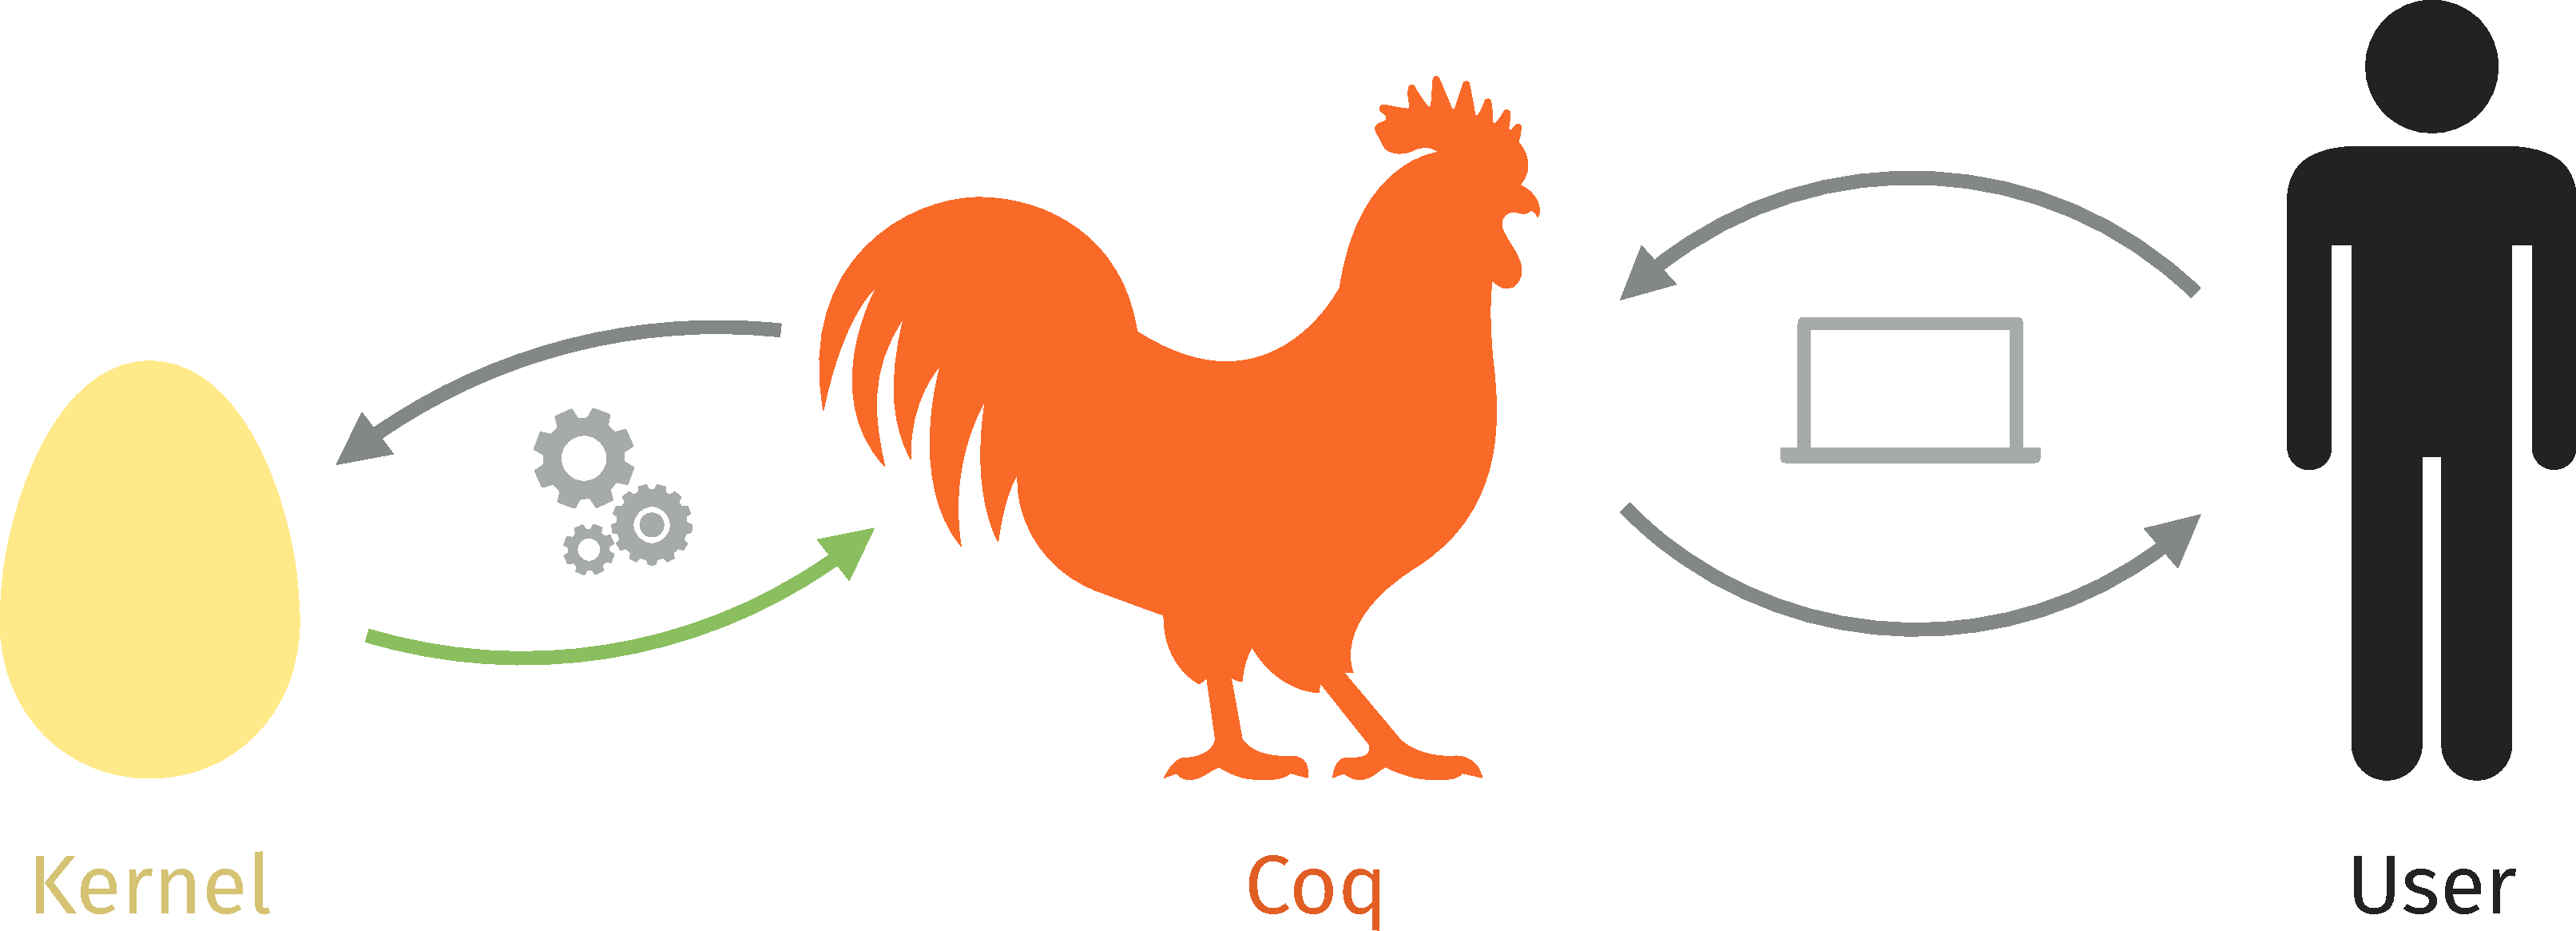
\includegraphics[width=0.99\textwidth]{coq-kernel.pdf}
\end{figure}

In this setting the kernel has to be kept as small as possible for inspection
by humans. In particular experimental features are dangerous in there.
\marginnote[0.1cm]{
  The interested reader can have a look at
  \url{https://github.com/coq/coq/blob/master/dev/doc/critical-bugs}
  where a list of critical bugs of \Coq is maintained.
}
Unfortunately, \Coq's kernel is not free of mistakes, and one critical bug has
been found roughly every year for the last two decades. Even then the kernel
presentation offers some damage control as it usually requires minor changes to
fix the problem.
In fact, those bugs are always related to the implementation rather than beeing
consistency issues of \acrshort{PCUIC}.

\acrshort{PCUIC} on the other hand seems more worthy of trust. The idea of our
project~\sidecite{sozeau2019coq} represents a paradigm shift: we propose to
replace the \acrshort{TCB} by a \acrfull{TTB}.
\begin{figure}[hb]
  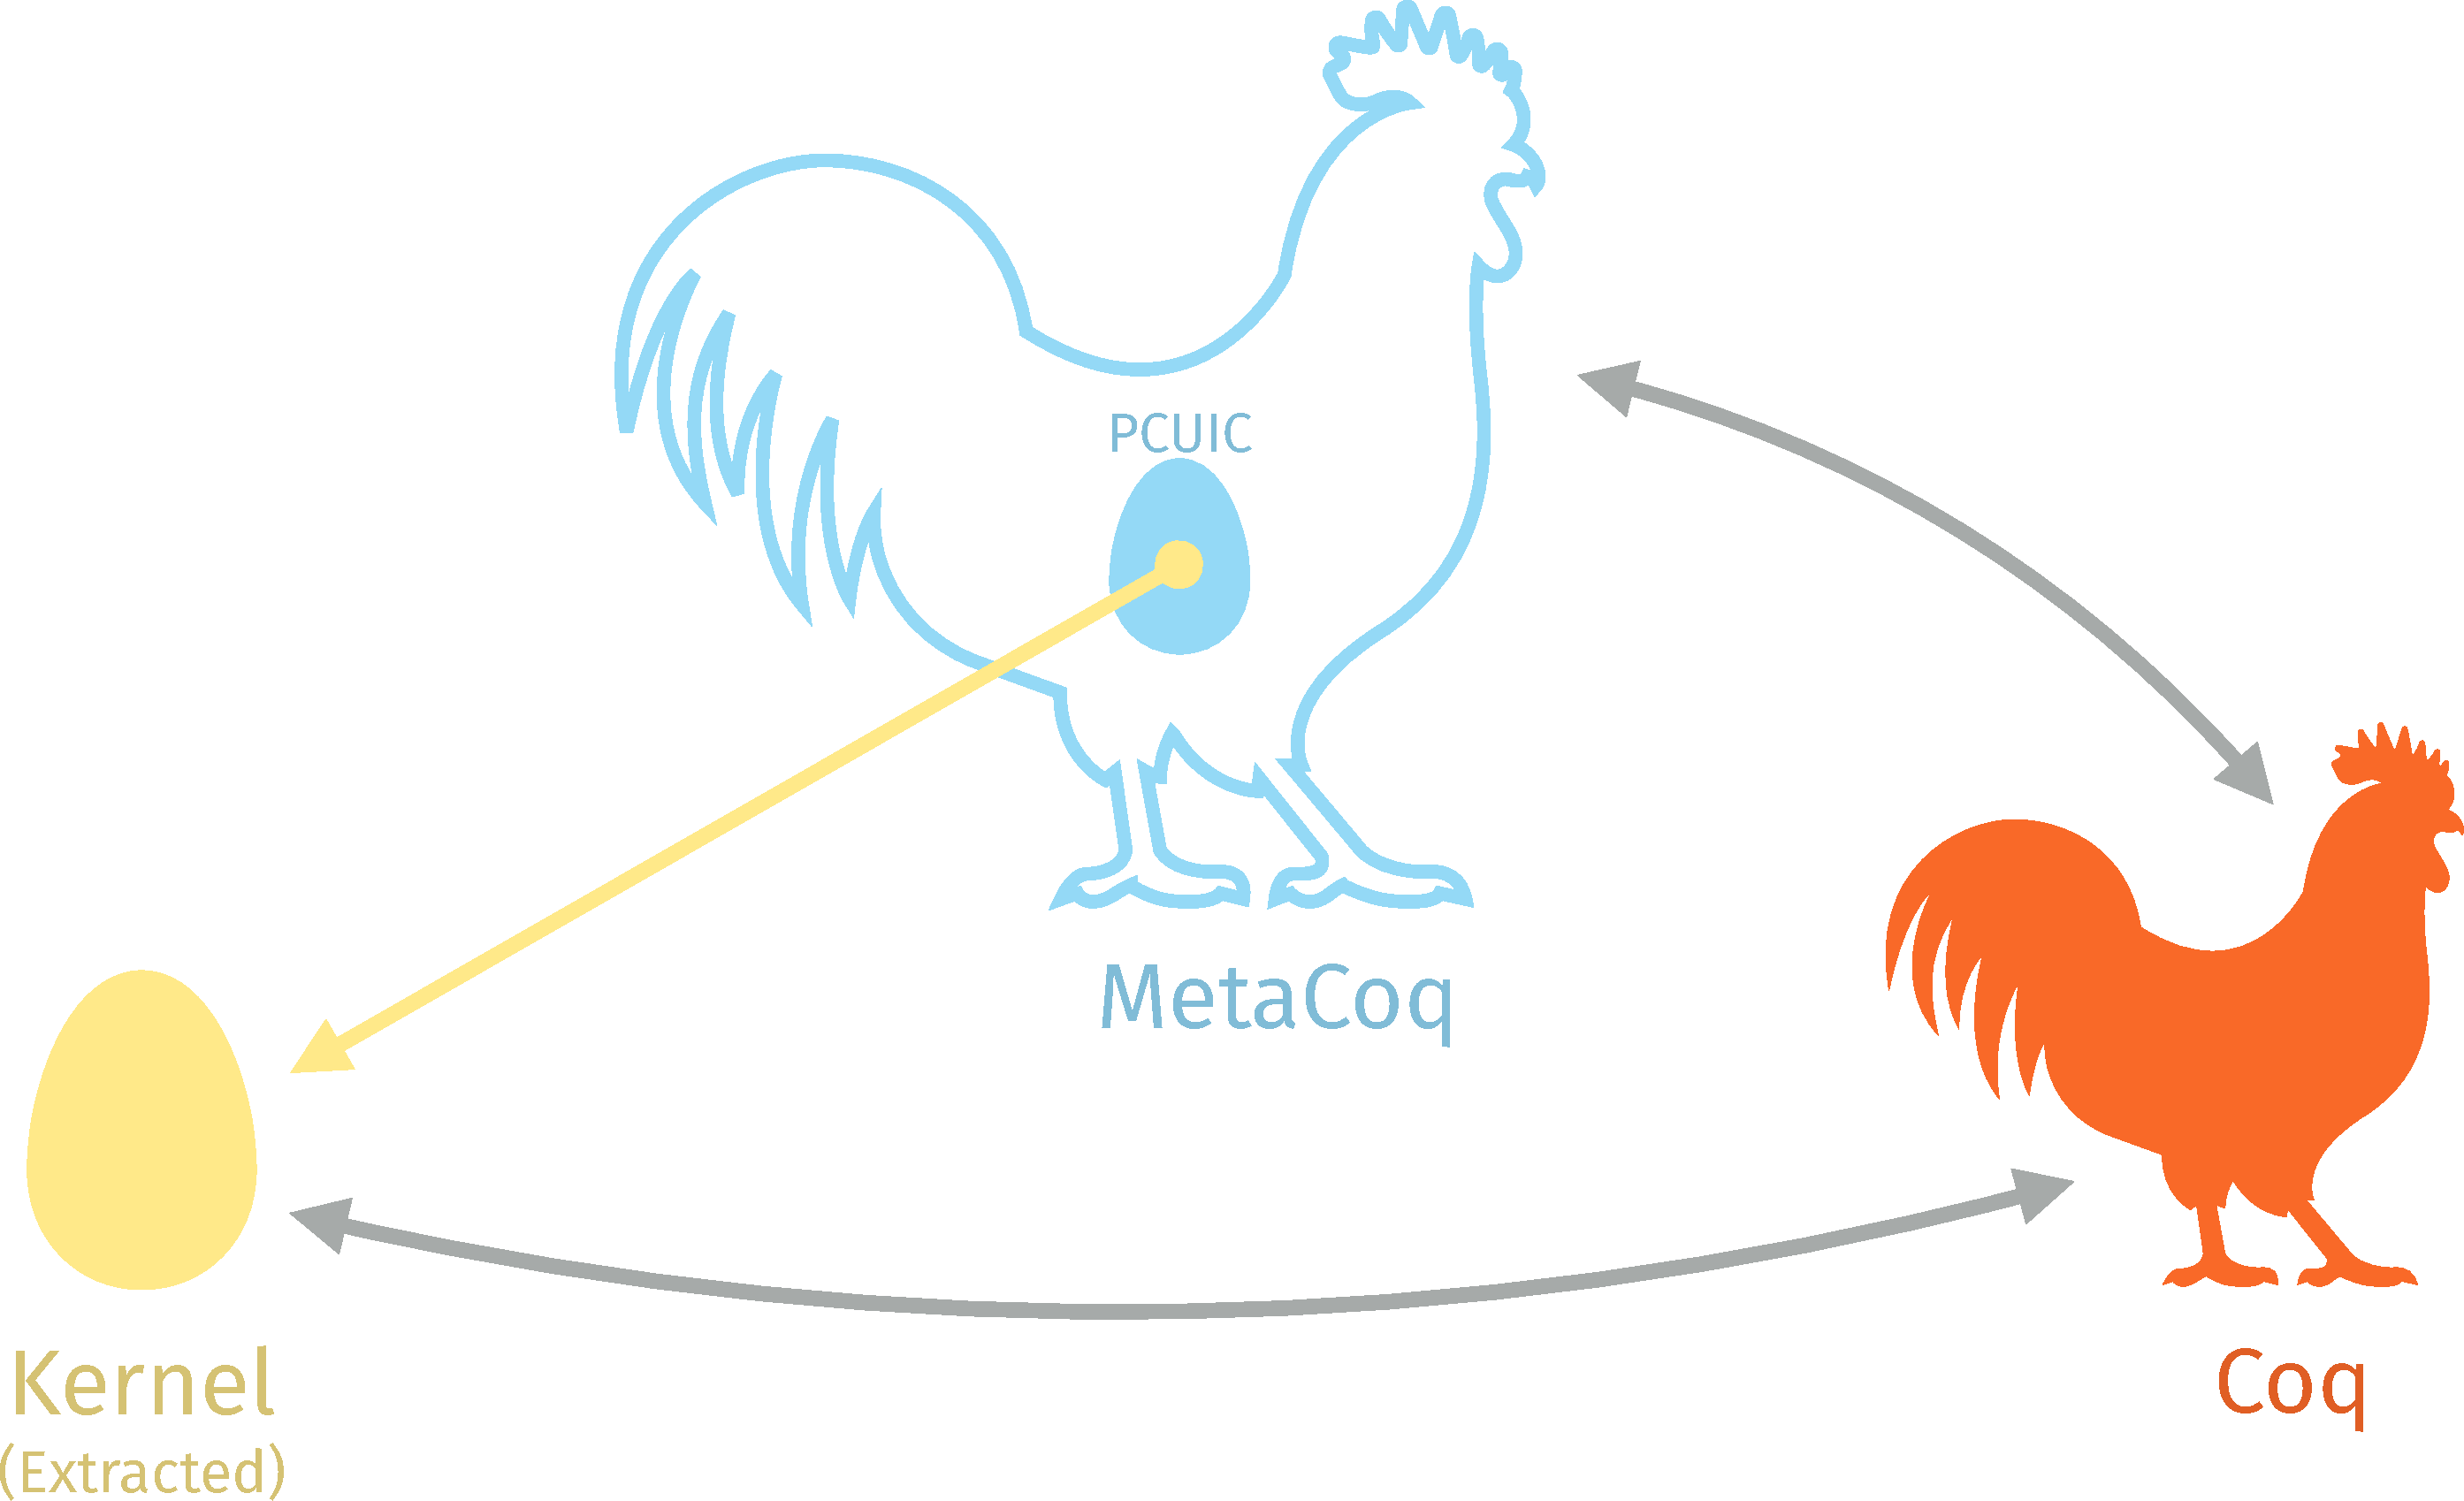
\includegraphics[width=0.7\textwidth]{trusted-theory.pdf}
\end{figure}

This time the idea is to rely on \MetaCoq which contains a specification of
\acrshort{PCUIC} to implement a verified kernel, assuming that the theory is
correct (hence the \acrshort{TTB}).
This \acrshort{TTB} is also kept to a minimum, only a few lemmata are part of it
now, and in time it should only consist in assuming strong normalisation.
The new kernel can be extracted to \Coq using its extraction
mechanism~\sidecite{Let2008} and it no longer has to be trusted. Of course this
requires trusting the extraction mechanism and even \Coq itself in which
\acrshort{PCUIC} is formalised.
The first point is mitigated by a verified extraction that is also part of the
project. The latter is more fundamental but I would like to argue that this is
\emph{not} entirely detrimental to our goal: the verified implementation is
still more detailed than the \ocaml implementation, in particular all the
invariants are made explicit; implementation and specification are now clearly
separated.

\marginnote[0.2cm]{
  See \nrefch{proof-theory} for more on Gödel's incompleteness theorems.
}
Note that we still have to rely on a \acrshort{TTB} because of Gödel's
incompleteness theorems which prevent us from proving consistency of
\Coq within \Coq.
\marginnote[0.1cm]{
  See \nrefch{desirable-props}.
}
This implies that we have to admit strong normalisation of the system, as it
would lead us to canonicity, hence consistency.
Thus, the assumption that the meta-theory enjoys the well-known assumed
properties is the main shortcoming of our formalisation. If those did not hold,
it would either raise a serious issue in \Coq's theory, or a problem in the
specification we made of it. For this last reason, the relatively small
specification we have is welcome.

\marginnote[1.2cm]{
  See \nrefch{flavours}.
}
Besides that, the theory of \acrshort{PCUIC} we specify and implement is a bit
simpler than that of \Coq: we use lists where arrays are involved and more
importantly we do not feature modules and template polymorphism.
The implementation also provides efficient universe constraint checking and
guard condition checking, we chose to remain abstract over those and simply
assume the existence of those in the specification: any implementation
satisfaying the specification can thus be plugged in. We use a rather naive
universe checker for now and do not provide any guard checking at all.